
    In the preceding chapter, a mathematical theory for contraint programming on
    static single assignment compiler intermediate representation was derived.
    This chapter will now build on top of this theoretical framework, developing
    a domain specific contraint programming language and presenting an
    implementation of this language in the production quality LLVM compiler
    infrastructure.

    The Compiler Analysis Description Language (CAnDL) makes it possible to
    automatically generate compiler analysis functions that would otherwise
    have to be implemented manually.
    Such a programming language fits an important niche in compiler development:
    Optimizing compilers utilise elaborate program transformations to exploit
    increasingly complex hardware, and implementing the appropriate analysis
    functionality for such optimizations to be safely applied is a time
    consuming and error prone activity.
    For example, tens of thousands of lines of code are required in the LLVM
    code base to detect the appropriate places to apply peephole optimizations
    and bugs in this functionality can result in corrupted user programs.
    This is a barrier to the rapid prototyping and evaluation of new
    optimizations.

    CAnDL enables a workflow that is much more amenable to efficient compiler
    development:
    The compiler implementer only has to write CAnDL programs, which are then
    compiled by the CAnDL compiler fully automatically into C++ LLVM passes.
    These passes automatically spot code sections that adhere the specified
    structure, leaving only the transformation functionality to be implemented
    by hand.
    This provides a uniform manner in which to describe compiler analysis,
    reducing code length and complexity.

    The approach crucially scales to a wide range of compiler analysis tasks,
    ranging from the detection of small scale local optimization opportunities
    over domain specific graphics optimizations to fully capturing polyhedral
    static control flow regions.
    In all cases, these tasks can be  expressed more briefly than with competing
    approaches.

\section{Introduction}

    Compilers are complex pieces of software responsible that proces source code
    in several stages to produce an efficient binary program.
    In order to generate fast programs, compilers rely on a complex mid end, in
    which program optimisations are applied to the user program after parsing
    and before code genreation.
    In this mid end, user code is typically represented in a static single
    assignment intermediate representation and is optimised by successively
    applying a wide range of optimization passes.
    There is generally obvious upper bound to the complexity of optimisations
    that are considered, instead compilers are limited by their increasing code
    complexity and by the necessity to reason at each stage about the soundness
    of the performed operations.
    It is crucial that optimisations retain the semantics of the original
    program, as otherwise the resulting binary might be compromised.
    

    Implementations of compiler optimizations generally require two components:
    analysis and transformation.
    Analysis routines find candidate sections in user programs that could profit
    from specific transformations and verify that all conditions are satisfied
    in order to legally apply them.
    Transformations are then applied to the analysis results, often after
    consulting heuristic cost models to gauge the effect on runtime, code size
    and other metrics.

    The analysis often contains much of the code complexity.
    For example, simple peephole optimizations in the LLVM {\tt instcombine}
    pass contain approximately 30000 lines of complex C++ code, despite the
    transformations being simple.
    This impedes the implementation of new compiler passes, preventing the rapid
    prototyping of new ideas.
    Furthermore, this is an important source of bugs and bugs in this stage of
    the compiler are particularly pernicious, as they tamper with the user
    programs.
    Ideally, we would like a simpler way of describing such analysis that
    reduces boiler-plate code and opens the way for new compiler optimization
    innovation in a controlled fashion.

    This chapter presents CAnDL, a domain specific language for compiler
    analysis.
    It is a constraint programming language that operates on the static single
    assignment intermediate representation of the LLVM compiler infrastructure
    (LLVM IR).
    Instead of writing compiler analysis code inside the main codebase of the
    compiler infrastructure, it enables compiler writers to specify optimization
    functionality external to the main C++ code base.
    The CAnDL compiler then generates C++ functions that are linked together
    with the clang compiler binary and that implement LLVM passs.
    The formulation of optimizing transformations in CAnDL is faster, simpler
    and less error prone than writing them in C++.
    It has a strong emphasis on modularity, which enables debugging and the
    formulation of highly readable code.

    The implementation of CAnDL is based on the constraint programming
    methodology that was introduced in \autoref{chapter:theory}, using a solver
    that is integrated directly into the LLVM code base.
    On top of this solver, a complete working system is provided, including a
    full parser and code generator for CAnDL as a full-fledged programming
    langauge.

\section{Example}

\begin{figure}[b]
\centering
\caption{Simple Declarative CAnDL Specificaiton}
\label{fig:candlspec}
\begin{minipage}[t]{0.67\textwidth}
\begin{lstlisting}[language=CAnDL]
Constraint SqrtOfSquare
( opcode{sqrt_call} = call
([$\tt \land$]) {sqrt_call}.args[0] = {sqrt_fn}
([$\tt \land$]) function_name{sqrt_fn} = sqrt
([$\tt \land$]) {sqrt_call}.args[1]  = {square}
([$\tt \land$]) opcode{square} = fmul
([$\tt \land$]) {square}.args[0] = {a}
([$\tt \land$]) {square}.args[1] = {a})
End
\end{lstlisting}
\end{minipage}
\end{figure}

    As an example of the CAnDL workflow, consider  \autoref{fig:root}.
    This basic algebraic equation can be interpreted as a recipe for a compiler
    optimisation:
    Assuming an environment without the particularities of floating point
    arithmetic (i.e.\ assuming the \texttt{-ffast-math} flag is active), the
    compiler could use this equality to eliminate some square root invocations
    in user code.
    This is desirable, as the square root has to be approximated with relatively
    expensive numerical methods, whereas computing the absolute value is
    computationally cheap.
    \begin{align}
    \label{fig:root}
    \forall a\in \mathbb{R}\colon\ \sqrt{a*a}=|a|
    \end{align}

    The compiler should use the equation left to right:
    It should analyse the user code in order to find representations of  the
    left side of the equation and then transform all those occurences analogous
    to the right side of the equation.
    The compiler therefor must detect occurrences of $\sqrt{a*a}$ in the LLVM IR
    code and replace them with a call to the \texttt{abs} function.
    The generation of the new function call is trivial, but the detection of
    even a simple pattern like $\sqrt{a*a}$ requires some care when implementing
    it manually in a complex code base such as LLVM.

    The established approach would be to implement it as part of the
    \texttt{instcombine} pass, which applies a collection of such peephole
    optimisations and already extends to almost 30000 lines of C++ code.
    This code makes heavy use of raw pointers and dynamic type casts and has
    been identified as a frequent source of bugs by
    \citet{Yang:2011:FUB:1993316.1993532, Menendez:2017:ADP:3062341.3062372}.
    This is impractical and an impediment to compiler development.

    Instead, CAnDL allows a declarative description of the analysis problem,
    which is easier to follow, has no interaction with other optimisations and
    is much less verbose.
    This is shown in \autoref{fig:candlspec}.
    The specification is given the identifier \texttt{SqrtOfSquare} in the
    first line of the program and then defined by the interaction of seven
    atomic constraint statements that have to hold simultaneously hold on the
    values of \texttt{sqrt\_call}, \texttt{sqrt\_fn}, \texttt{square} and
    \texttt{a}.
    The lines 2-8 each stipulate one of these constraints and they are joined
    together with the logical conjunction operator ``$\land$''.

    The CAnDL compiler translates this declarative program into a C++ analysis
    function that is used as an LLVM optimisation pass.
    This is demonstrated in \autoref{fig:candlexample}, which shows the analysis
    function generated from the CAnDL specification in \autoref{fig:candlspec}
    applied to a user program ({\bf a}-{\bf d}).
    The input program ({\bf a}) is a simple C program that calls the
    \texttt{sqrt} function twice with squares of floating point values.
    It is translated using the clang compiler into LLVM IR code ({\bf b}),
    applying standard optimisation passes during the process.
    This results in the expressions from the user program being sequentialised,
    with the two occurences of the \texttt{SqrtOfSquare} idiom clearly visible:
    The two \texttt{fmul} instructions compute squares via a floating point
    multiplication and these are then used as arguments to \texttt{sqrt}
    function invocations. 

    The analysis function detects two opportunities to apply the transformation,
    shown as first solution ({\bf d}) and second solution ({\bf e}).
    Each of the two solutions assigns values from within the LLVM IR code to
    each of the variables in the CAnDL program such that all the specified
    constraints are fulfilled.
    The validity of these solutions is demonstrated in the middle row of the
    figure ({\bf e}-{\bf f}).
    Subsituting the variables in the CAnDL programs with the concrete
    instantiations from the solutions, we can verify the individual atomic
    constraints one by one:
    \begin{itemize}
    \item \texttt{\%4} and \texttt{\%6} are function calls and their first
          argument (the function to be called) is \texttt{@sqrt}.
    \item \texttt{@sqrt} is the square root function.
          Note that we have no choice but to identify it by name.
    \item The second argument of the function call instruction (and hence the
          first actual function argument) are \texttt{\%3} and \texttt{\%5}
          respectively.
    \item \texttt{\%3} and \texttt{\%5} are square values, i.e.\ a floating
          point multiplication of a value with itself.
    \end{itemize}

    With the solutions identified by the CAnDL system, performing the
    transformation is now simple.
    The result of the analysis for each solution is provided in the form of a
    C++ dictionary \texttt{std::map<std::string,llvm::Value*>}, which contains
    the information required to apply appropriate code transformations
    ({\bf g}).
    A new function call to \texttt{abs} is generated, with \texttt{a} as the
    only argument.
    This instruction then replaces the original call instruction that was
    captured in \texttt{sqrt\_call}.
    After post processing with standard dead code elimination, this results in
    the optimized code shown at the bottom of the figure ({\bf h}).

    Although this is only a small example, it illustrates the main steps of the
    CAnDL scheme.
    In practice, the strength of the system is to scale to complex
    specifications, culminating in a full polyhedral analysis, which will be
    demonstrated towards the end of the chapter.
    The next sections give a specification of the CAnDL language and outline how
    it is implemented on top of the constraint programming methodology devised
    in \autoref{chapter:theory}.

\begin{figure*}[p]
    \centering
\begin{minipage}[t]{0.67\textwidth}
\centering
{\bf(a)} CAnDL program:
\begin{lstlisting}[language=CAnDL]
Constraint SqrtOfSquare
( opcode{sqrt_call} = call
([$\tt \land$]) {sqrt_call}.args[0] = {sqrt_fn}
([$\tt \land$]) function_name{sqrt_fn} = sqrt
([$\tt \land$]) {sqrt_call}.args[1]  = {square}
([$\tt \land$]) opcode{square} = fmul
([$\tt \land$]) {square}.args[0] = {a}
([$\tt \land$]) {square}.args[1] = {a})
End
\end{lstlisting}
\end{minipage}

\vspace{1em}
\begin{minipage}[t]{\textwidth}
\centering
\begin{minipage}[t]{\textwidth}
\centering
{\bf(b)} C program code:
\begin{lstlisting}[numbers=none,framexleftmargin=0pt,xleftmargin=0pt,language=C,basicstyle=\small\ttfamily]
 double example(double a, double b) {return sqrt(a*a) + sqrt(b*b); }
\end{lstlisting}
\end{minipage}
\begin{minipage}[t]{7.1cm}
\centering
{\bf(c)} Resulting LLVM IR:
\begin{lstlisting}[language={LLVM}]
define double @example(    
 double %0,                
 double %1) {              
 %3 = fmul double %0, %0   
 %4 = call double @sqrt(%3)
 %5 = fmul double %1, %1   
 %6 = call double @sqrt(%5)
 %7 = fadd double %4, %6   
 ret double %7 }
declare double @sqrt(double)      
\end{lstlisting}
\end{minipage}
\hfill
\begin{minipage}[t]{3.5cm}
\centering
{\bf(d)} First solution:
\begin{lstlisting}[numbers=none,framexleftmargin=0pt,xleftmargin=0pt,language=LLVM]

a = %0

square = %3
sqrt_call = %4 




sqrt_fn = @sqrt
\end{lstlisting}
\end{minipage}
\hfill
\begin{minipage}[t]{3.5cm}
\centering
{\bf(e)} Second solution:
\begin{lstlisting}[numbers=none,framexleftmargin=0pt,xleftmargin=0pt,language=LLVM]


a = %1


square = %5
sqrt_call = %6


sqrt_fn = @sqrt
\end{lstlisting}
\end{minipage}
\end{minipage}


\vspace{1em}
\begin{minipage}[t]{\textwidth}
\centering
{\bf(f)} C++ transformation code:
\begin{lstlisting}
void transform(map<string,Value*> solution, Function* abs) {
    ReplaceInstWithInst(
       dyn_cast<Instruction>(solution["sqrt_call"]),
       CallInst::Create(abs, {solution["a"]}));
}
\end{lstlisting}
\end{minipage}

\vspace{1em}
\begin{minipage}[t]{\textwidth}
\centering
{\bf(g)} Transformed LLVM IR after DCE:
\begin{lstlisting}[escapeinside={(*}{*)},language={LLVM}]
define double @example(double %0, double %1) {              
 %3 = call double @abs(double %0) 
 %4 = call double @abs(double %1)
 %5 = fadd double %3, %4   
 ret double %5 }
\end{lstlisting}
\end{minipage}

\caption{Demonstration of a simple CAnDL specification ({\bf a}) on an example C
         program ({\bf b}):
         In the generated LLVM intermediate code ({\bf c}), two instances
         ({\bf d},{\bf e}) of {\tt SqrtOfSquare} are detected.
         Applying an optimization using these results is trivial ({\bf g}) and
         results in efficient code ({\bf e}).}
    \label{fig:candlexample}
\end{figure*}

\section{Language Specification}

    The Compiler Analysis Description Language (CAnDL) is a domain specific
    programming language for the specification of compiler analysis
    passes. 
    Individual CAnDL programs define computational structures to be exploited by
    optimizing code transformations.
    These structures are specified as constraints on static static assignment
    (SSA) form representations of programs.

    The expressed structures can scale from simple instruction patterns that are
    suited for peephole optimizations over basic control flow structures such as
    loops to complex algorithmic concepts such as stencil codes with arbitrary
    kernel functions or code regions suitable for polyhedral analysis.

    The basic building blocks of CAnDL programs are well known compiler analysis
    tools, such as constraints on data and control flow, data types and
    instruction opcodes.
    On top of these low level constraints, CAnDL employs powerful mechanisms for
    modularity and encapsulation that allow the construction of complex
    programs.

\subsection{High Level Structure of CAnDL Programs}

    An individual CAnDL program contains constraint formulas that are
    bound to identifiers.
    As we already saw in \autoref{fig:firstexample} (a), the syntax for this is
    as follows:
    \begin{align*}
        \text{\bf Constraint}\ \left<\text{\bf s}\right>\ \text{\it formula}\ \text{\bf End}
    \end{align*}
    For the description of CAnDL syntax we use these notational conventions:
    terminal symbols are {\bf bold}, non-terminals are {\it italic},
    $\left<\text{\bf s}\right>$ is an identifier (alphanumeric string) and
    $\left<\text{\bf n}\right>$ is an integer literal.

    We already saw in \autoref{fig:firstexample} (a) that logical conjunctions
    can be used to combine {\it formula}s.
    More generally, a {\it formula} can be any of the following:
    \begin{align*}
        &\text{\it atomic}\mid\text{\it conjunction}\mid \text{\it disjunction}\\
        \mid{}&{}\text{\it foreach}\mid \text{\it forany}\mid\text{\it include}\mid\text{\it collect}
    \end{align*}
    The basis of every CAnDL program are {\it atomic} constraints.
    For example in \autoref{fig:firstexample} (a), lines 2-8 each specify
    individual atomic constraints.
    Atomic constraints are bound together by logical connectives $\land$ and
    $\lor$ ({\it conjunction} and {\it disjunction}) and other higher level
    constructs.
    These include two kinds of loop structures ({\it foreach}, {\it forany}), as
    well as a system for modularity (\texttt{include}).
    Lastly, the {\it collect} construct allows for the formulation of more
    complex constraints that require the $\forall$ quantifier.

\subsection{Atomic Constraints}

    The first type of constraint is an {\it atomic} constraint based on
    {\it variable}s.
    {\it Variable}s in CAnDL correspond to instructions and values in LLVM IR. 
    Given some IR code, all occurring values can be assigned to the
    {\it variable}s of a given constraint formula.
    This includes instructions, globals, constants and function parameters.
    Syntactically, a variable is simply an identifier in curly brackets.

    CAnDL uses the following atomic constraints:
    \begin{align*}
        \text{\bf data\_type}\ \text{\it variable}\ &\text{\bf =}\ \text{\bf int}\\
        \text{\bf data\_type}\ \text{\it variable}\ &\text{\bf =}\ \text{\bf float}
    \end{align*}
    This restricts the data type to integer or floating point.
    \begin{align*}
        \text{\bf ir\_type}\ \text{\it variable}\ &\text{\bf =}\ \text{\bf literal}\\
        \text{\bf ir\_type}\ \text{\it variable}\ &\text{\bf =}\ \text{\bf argument}\\
        \text{\bf ir\_type}\ \text{\it variable}\ &\text{\bf =}\ \text{\bf instruction}
    \end{align*}
    This restricts the type of IR node that is allowed to compile time constants, function arguments or instructions.
    \begin{align*}
        \text{\bf opcode}\ \text{\it variable}\ &\text{\bf =}\ \left<\text{\bf s}\right>
    \end{align*}
    This restricts the value instructions of the specified opcode.
    \begin{align*}
        \text{\bf function\_name}\ \text{\it variable}\ \text{\bf =}\ \left<\text{\bf s}\right>
    \end{align*}
    This restricts the variable to be a specified standard function (i.e.\ the {\tt sqrt} function).
    \begin{align*}
        \text{variable}\ &\text{\bf =}\ \text{variable}\\
        \text{variable}\ &\text{\bf !=}\ \text{variable}
    \end{align*}
    This enforces two variables to have the same/not the same value.
    This is a shallow comparison, i.e. it compares whether two variables represent the same IR node. 
    \begin{align*}
        \text{\bf control\_origin}&\ \text{\it variable}\\
        \text{\bf data\_origin}&\ \text{\it variable}
    \end{align*}
    The value is an origin of control (function entry) or data (function argument, {\tt load} instruction, inpure function call).
    \begin{align*}
        \text{\it variable}\text{\bf.arg[}\left<\text{\bf n}\right>{\bf]}\ &\text{\bf =}\ \text{\it variable}\\
        \text{\it variable}\ &\text{\bf $\in$}\ \text{\it variable}\text{\bf .args}
    \end{align*}
    There data flow from one value to the next.
    \begin{align*}
        \text{\it variable}\ \text{\bf ->}\ \text{\it variable}\ \Phi\ \text{\it variable}
    \end{align*}
    The left value has to reach the right value, which is a phi node, via the middle value, which is a jump instruction.
    \begin{align*}
        \text{\bf domination(}\text{\it variable}\text{\bf,} \text{\it variable}\text{\bf)}&\\
        \text{\bf strict\_domination(}\text{\it variable}\text{\bf,} \text{\it variable}\text{\bf)}&
    \end{align*}
    Both values have to be instructions and the first dominates the second in the control flow graph.
    \begin{align*}
        \text{\bf calculated\_from(}\text{\it varlist}\text{\bf,}\text{\it varlist}\text{\bf,}\text{\it variable}\text{\bf)}
    \end{align*}
    {\it Varlist} is a set of one or multiple {\it variables}.
    Any path from one of the entries in the first {\it varlist} to the single
    {\it variable} argument has to pass through at least one of the entries in
    the second {\it varlist}.
    All paths in the union of the data flow and control dependence graph are
    considered.
    We will see later how this is useful to specify kernel functions for
    e.g.\ stencil calculations.

    There are some {\it atomic}s that we omit for space reasons.
    The set of {\it atomic}s that CAnDL supports is easily extensible.
    Possible additions include constraints on function attributes, value
    constraints on literals etc.

\subsection{Range Constraints}

    Building on top of the basic conjunction and disjunction constructs, there
    are range based versions that operate on arrays of variables.
    \begin{align*}
        \text{\it formula}\ &\text{\bf foreach}\ \left<\text{\bf s}\right>\ \text{\bf =}\ \text{\it index}\ \text{\bf ..}\ \text{\it index}\\
        \text{\it formula}\ &\text{\bf forany}\ \left<\text{\bf s}\right>\ \text{\bf =}\ \text{\it index}\ \text{\bf ..}\ \text{\it index}
    \end{align*}
    These constructs allow the repeated application of a formula according to
    some range of indices.
    This is demonstrated by \autoref{fig:forall}, which shows two equivalent
    CAnDL programs, one formulated with \texttt{foreach} and one without.
    In both cases, the program specifies an array of five variables with data
    flow from each element to the next.
    We can see how the \texttt{foreach} loop can be expanded similar to loop
    unrolling.

    UNDERFUL VBOX.

    UNDERFUL VBOX.

\begin{figure}[ht]
\begin{lstlisting}[language=CAnDL]
Constraint ValueChain
 {element[i] ([$\tt \in$]) {element[i+1]}.args foreach i=0..4
End
\end{lstlisting}
\begin{lstlisting}[language=CAnDL]
Constraint ValueChain
( {element[0]} ([$\tt \in$]) {element[1]}.args
([$\tt \land$]) {element[1]} ([$\tt \in$]) {element[2]}.args
([$\tt \land$]) {element[2]} ([$\tt \in$]) {element[3]}.args
([$\tt \land$]) {element[3]} ([$\tt \in$]) {element[4]}.args)
End
\end{lstlisting}
\vspace{-0.3cm}
\caption{Expansion of range constraints in CAnDL}
\label{fig:forall}
\end{figure}

\subsubsection{Modularity}
    \label{sec:modularity}

    Modularity is central to the CAnDL programming language, and it is achieved
    using the {\it include} construct.
    \begin{align*}
        \text{\bf include}\ &\left<\text{\bf s}\right>\\
                            &[\text{\bf (}\text{\it variable}\ \text{\bf ->}\ \text{\it variable}\ \{\text{\bf ,}\ \text{\it variable}\ \text{\bf ->}\ \text{\it variable}\}\text{\bf )}]\\
                            &[\text{\bf @}\ \text{\it variable}]
    \end{align*}
    Note that the syntax in square brackets is optional and the syntax in curly
    brackets can be repeated.
    The basic version of \texttt{\it include}, without the optional structures,
    is simple.
    It copies the {\it formula} that corresponds to the identifier verbatim into
    another {\it formula}.
    If $[\text{\bf @}\ \text{\it variable}]$ is specified, then all the variable
    names of the inserted constraint formula are prefixed with the given
    variable name, separated with a dot.
    The other optional syntax is used to rename individual {\it variable}s in
    the included {\it formula}.

    \autoref{fig:inheritsandrenameandrebase} illustrates this with two
    equivalent programs.
    Both programs specify an addition of four values, first adding pairwise and
    then adding the intermediate results.
    We can see in the first listing that a {\it formula} for the addition of two
    values is bound to the name {\tt Sum}.
    This is then included three times in another {\it formula} names
    {\tt SumOfSums}.
    Using the optional grammatical constructs, the formula operates on a
    different set of {\it variable}s each time such that the third addition
    takes the results of the previous two as input.

\begin{figure}[ht]
\lstset{
 basicstyle = \linespread{0.88}\ttfamily
}
\begin{lstlisting}[language=CAnDL]
Constraint Sum
( opcode{out} = add
∧ {in1} = {out}.args[0]
∧ {in2} = {out}.args[1])
End
Constraint SumOfSums
( include Sum@{sum1}
∧ include Sum@{sum2}
∧ include Sum({sum1.out}->{in1},{sum2.out}->{in2}))
End
\end{lstlisting}
\begin{lstlisting}[language=CAnDL,
                   label={fig:inheritsandrenameandrebase},caption=
   {Example for the expansion of {\it include} structure:
    Both specifications are equivalent.
    \leftskip=0pt\rightskip=0pt}]
Constraint SumOfSums
( opcode{sum1.out} = add
∧ {sum1.in1} = {sum1.out}.args[0]
∧ {sum1.in2} = {sum1.out}.args[1]
∧ opcode{sum2.out} = add
∧ {sum2.in1} = {sum2.out}.args[0]
∧ {sum2.in2} = {sum2.out}.args[1]
∧ opcode{out} = add
∧ {sum1.out} = {out}.args[0]
∧ {sum2.out} = {out}.args[1])
End
\end{lstlisting}
\label{fig:inheritsandrenameandrebase}
\end{figure}

\subsubsection{Collect}

    The \text{\it collect} construct is used to capture all possible solutions
    of a given formula.
    It is used to implement constraints that require the logical $\forall$
    quantifier.
    For example, it can be used to guarantee that all memory accesses in a loop
    use affine index computations.
    The grammar is simple but the semantics require some elaboration.
    \begin{align*}
        \text{\bf collect}\ \left<\text{\bf s}\right>\ \text{\it index}\ \text{\it formula}
    \end{align*}
    In \autoref{fig:simplecollect}, the variables \texttt{arg[0],\dots,arg[N-1]}
    are constraint to contain all of the data dependences of \texttt{ins}.
    The first argument of \text{\it collect} specifies the name of an index
    variable that is used to detect which variables belong to the collected set.
    In this example we want all solutions of \texttt{arg[i]} for a given value
    of \texttt{ins}.
    The second argument gives an upper bound to the amount of collected
    variables, in this case we leave it unspecified by using the symbol
    \texttt{N}.

\begin{figure}[ht]
\begin{lstlisting}[language=CAnDL]
Constraint CollectArguments
( ir_type{ins} = instruction
([$\tt \land$]) collect i N ({arg[i]} ([$\tt \in$]) {ins}.args))
End
\end{lstlisting}
\vspace{-0.3cm}
\caption{Simple collect example in CAnDL}
\label{fig:simplecollect}
\end{figure}

    We can now extend this example to show how {\it collect} can be used to
    implement quantifiers.
    Consider that we want to detect instructions with only floating point data
    dependences.
    This involves the $\forall$ quantifier, as it is equivalent to
    the following equation.
    \begin{align}
        \forall v\colon\ v\in I.\text{args}\implies\text{data\_type}(v)=\text{float}
    \label{fig:implication}
    \end{align}
    We can rewrite this to an equivalent formulation on sets.
    \begin{align*}
        S_1:= \{v\mid v\in I.\text{args}\}\subset S_2:={}\{v\mid\text{data\_type}(v)=\text{float}\}
    \end{align*}
    Now we can apply the following equivalences:
    \begin{align*}
        &S_1\subset S_2\Leftrightarrow{}S_1 = S_1\cap S_2\\
        \Leftrightarrow{}&\exists S\colon S=S_1\land S=S_1\cap S_2
    \end{align*}
    This means that if we constraint a set $S$ to be equal to both $S_1$ and
    $S_1\cap S_2$ at the same time, the constraints are satisfiable if and only
    if the implication in \autoref{fig:implication} holds.

    This condition can be expressed in CAnDL, as is shown in
    \autoref{fig:collectexample}.
    With the first {\it collect} statement in line 3, we constrain the set
    \texttt{arg} to be equal to $S_1$ and with the second one in lines 4-5 we
    constrain it to be $S_1\cap S_2$ as well.
    Note that we were from the onset only interested in the values that qualify
    for \texttt{ins}.
    The set \texttt{arg} was only introduced to further constraint \texttt{ins},
    not because we actually wanted to know the values that it contains.

\begin{figure}[ht]
\begin{lstlisting}[language=CAnDL]
Constraint FloatingPointInstruction
( ir_type{ins} = instruction
([$\tt \land$]) collect i N ( {ins} ([$\tt \in$]) {arg[i]}.args)
([$\tt \land$]) collect i N ( {ins} ([$\tt \in$]) {arg[i]}.args
              ([$\tt \land$]) data_type{arg[i]} = float))
End
\end{lstlisting}
\vspace{-0.3cm}
\caption{Collect Example in CAnDL}
\label{fig:collectexample}
\end{figure}

    The exact same approach can be used to e.g. restrict all array accesses in a
    loop to be affine in the loop iterators.
    This can be achieved by first {\it collect}ing all memory accesses
    (i.e.\ all \texttt{load} and \texttt{store} instrutions) and then using
    another {\it collect} statement to stipulate affine calculations for the
    indices.

\subsection{Expressing Larger Structures}

    The modularity of CAnDL allows the creation of a library of building blocks
    that are shared by multiple CAnDL programs.
    We will now give an overview about how these can be defined with CAnDL.

    Important building blocks include control flow structures such as single
    entry single exit regions and loops.
    These are standard in compiler analysis and the implementation in CAnDL is
    straightforward.
    A for loop involves a comparison of the loop iterator with the end of the
    iteration space.
    In order to be valid, this value has to be determined before the loop is
    entered, it isn't allowed to change from loop iteration to iteration.
    This leaves it to be either a function argument, an actual constant or an
    instruction that strictly dominates the loop entry.
    This is expressed in \autoref{fig:localconstant}.
    Note that this formula is to be included into larger CAnDL programs, as the
    \texttt{begin} variable is under specified otherwise.

\begin{figure}[ht]
\begin{lstlisting}[language=CAnDL]
Constraint LocalConst
( ir_type{value} = literal
([$\tt \lor$]) ir_type{value} = argument
([$\tt \lor$]) strict_domination({value}, {begin}))
End
\end{lstlisting}
\vspace{-0.3cm}
\caption{LocalConst in CAnDL}
\label{fig:localconstant}
\end{figure}

    Another class of important building blocks are different categories of
    memory access.
    These form a hierarchy of restrictiveness and include multidimensional array
    access and array access that is affine in some loop iterators.
    LLVM strictly separates memory access from pointer computations, which means
    that CAnDL only has to concern itself with plain pointer computations here.
    In general it is required that the base pointer is \texttt{LocalConst} in
    order to avoid pointer chases.
    The index computation can then be described using the data flow and
    instruction opcode restrictions.

    To enable the capture of higher order functions such as stencils or
    reduction operations, we need to handle arbitrary kernel functions.
    Kernel functions are sections of code that are side-effect free and
    can be separated out. Identifying side-effect free code is useful in
    many types of compiler optimization.  It can be expressed in CAnDL, as
    shown in \autoref{fig:kernel}.

\begin{figure}[ht]
\begin{lstlisting}[language=CAnDL]
Constraint KernelFunction
( collect i N
([$\tt \land$]) ( include LocalConst({outer}->{begin}*@*{closure[i]}
  ([$\tt \land$]) ir_type{closure[i].value} != literal
  ([$\tt \land$]) {closure[i].use} ([$\tt \in$]) {closure[i].value}.args
  ([$\tt \land$]) domination({inner}, {closure[i].use}))
([$\tt \land$]) collect i N data_origin{tainted1[i]}
([$\tt \land$]) collect i N
([$\tt \land$]) ( domination({outer}, {tainted2[i]})
  ([$\tt \land$]) strict_domination({tainted2[i]}, {inner}))
([$\tt \land$]) calculated_from(
   {tainted1[0..N],tainted2[0..N]},
   {origin[0..N],closure[0..N].value,input[0..N]},
   {output}))
End
\end{lstlisting}
\vspace{-0.3cm}
\caption{CAnDL Formulation of Kernel Functions}
\label{fig:kernel}
\end{figure}

    Essentially, this set of contraints captures the computation of a
    single \texttt{output} value from a set of specified \texttt{input}
    values as well as a set of automatically captured \texttt{closure}
    variables.  The computation for \texttt{output} should be such that it
    can be replaced with a function call that is free of side effects and
    takes only the \texttt{input} and \texttt{closure} variables as
    arguments.

    In addition to these variables, there are two non-obvious additional
    variables involved: \texttt{outer} and \texttt{inner}.
    These set boundaries in the control flow as follows: Closure values have to
    be computed before \texttt{outer} and the computation that results in outer
    is performed after \texttt{inner}.
    Usually these will be derived from loops nests, where \texttt{outer} is the
    entry to the outermost loop and \texttt{inner} is the entry to the innermost
    loop.
    The actual core constraint is then a generalized dominance relationship in
    the program dependence graph.

    The use of the sets \texttt{tainted1} and \texttt{tainted2} makes sure that
    no impure functions are used in computing \texttt{output} and the entire
    computation is performed after \texttt{inner} (ruling out e.g.\ loop carried
    variabls from outer loops).

    UNDERFUL VBOX.

    UNDERFUL VBOX.

    UNDERFUL VBOX.

\section{Implementation}

    CAnDL interacts with the LLVM framework, as shown in \autoref{fig:build2}.
    CAnDL programs are read by the CAnDL compiler, which then generates C++
    source code to implement the specified LLVM analysis functionality.
    This code depends on a generic backtracking solver, which is incorporated
    into the main LLVM code base. 
    We will see in the evaluation section this this solver adds little
    compile-time overhead in practice.
    The generated code is compiled and linked together with the existing LLVM
    libraries to make LLVM optimization passes available in the clang compiler.

    The generated analysis passes use the solver to search for the specified
    computational structures and output the found instances into report files,
    as well as making them available to ensuing transformation passes.

\begin{figure}[ht]
\centering
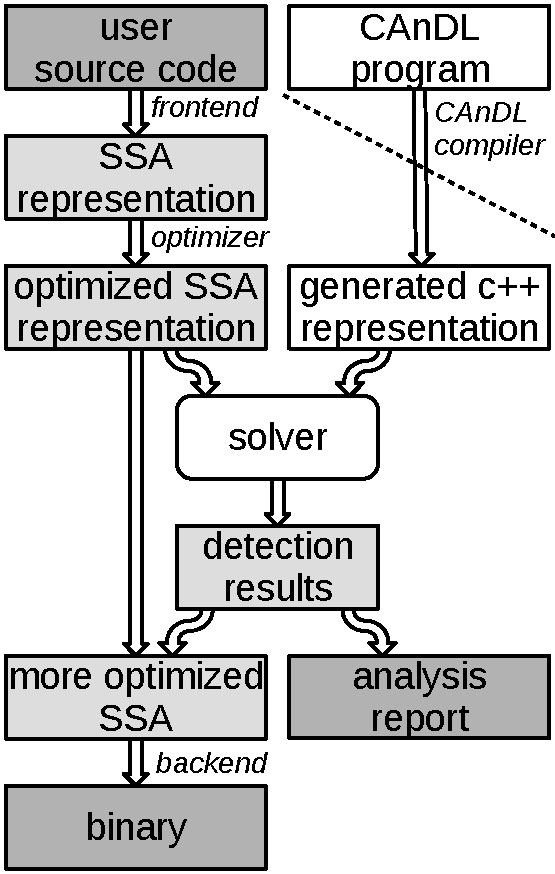
\includegraphics[width=0.29\textwidth]{figures/compilerFlow2.pdf}
\caption{CAnDL in the LLVM/clang build system}
\label{fig:build2}
\end{figure}

\subsection{The CAnDL Compiler}

\begin{figure}[t]
\centering
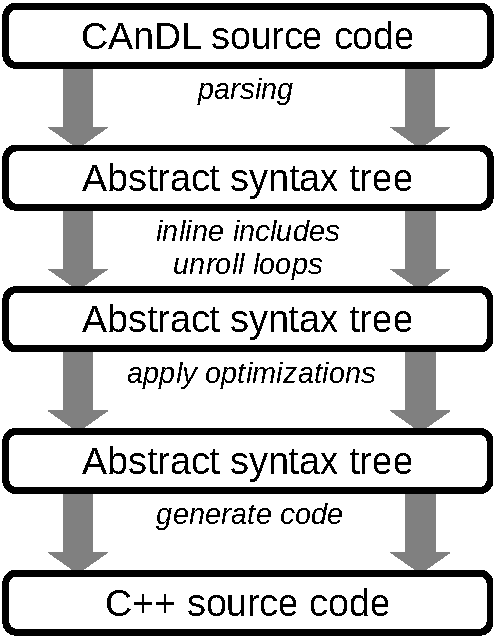
\includegraphics[width=0.29\textwidth]{figures/candlstages.pdf}
\caption{CAnDL compiler flow}
\label{fig:compilerflow}
\end{figure}

    The CAnDL compiler is responsible for generating C++ code from CAnDL
    programs.
    An overview of its  flow is shown in \autoref{fig:compilerflow}.
    The frontend reads in  CAnDL source code and builds an abstract syntax tree.
    This syntax tree is simplified in two steps to eliminate some of the higher
    order constructs of CAnDL.
    The \texttt{inheritance} clauses are replaced using standard function
    inlining after the contained variables have been transformed accordingly.
    Also, \texttt{foreach} and \texttt{forany} statements are lowered to
    conjunction and disjunction constructs by duplicating the contained constraint code
    and then renaming the contained variable names appropriately for each
    iteration. This is equivalent to complete loop unrolling.
    From this point onwards, variable names are treated as flat strings.
    The remaining core language now consists only of atomics, conjunctions,
    disjunctions and collections.

    The CAnDL compiler applies a set of basic optimizations to speed up the
    solving process using the later generated C++ code.
    For example, nested conjunctions and disjunctions are flattened wherever
    possible.

    Finally, the compiler generates the C++ source code.
    This essentially involves constructing the constraint problem as a graph
    structure that is accessible to the solver.

\subsubsection{C++ Code Generation}

    We demonstrate the code generation process in \autoref{fig:codegen} with an
    example.
    Each of the atomic constraints results in a line of C++ code that constructs
    an object of a corresponding class:
    In this case, the three involved atomic constraints are implemented by
    \texttt{AddInstruction}, \texttt{FirstArgument} and \texttt{SecondArgument}.
    For constraints that involve more than one variable, these objects are
    instantiated as shared pointers.

    The compiler then generates similar objects for the
    \texttt{conjunction}, \texttt{disjunction} and the \texttt{collect} structures.
    In our example, this only affects the variable \texttt{addition}, which is
    part of a \texttt{conjunction} clause.
    This results in an additional object construction that instantiates the
    \texttt{And} class corresponding to the {\bf $\land$} operator in CAnDL.
    The \texttt{select} function is used here to specify which variable of a
    constraint is being operated on.
    In this case, \texttt{addition} is the second variable in lines 3-4 of the
    CAnDL program, so we use \texttt{select<1>}.

    Finally, the generated objects are inserted into a vector together with the
    corresponding variable names.
    This vector is then passed to the solver.

\begin{figure}[ht]
\centering
\begin{lstlisting}[language=CAnDL]
Constraint SimpleAddition
( opcode{addition} = add
([$\tt \land$]) {addition}.args[0] = {left}
([$\tt \land$]) {addition}.args[1] = {right})
End
\end{lstlisting}
\begin{lstlisting}[language=C++]
auto constr0 = AddInstruction(context);
auto constr1 = make_shared<FirstArgument>(context);
auto constr2 = make_shared<SecondArgument>(context);
auto constr3 = And(constr0, select<1>(constr1),
                            select<1>(constr2));

vector<pair<string,SolverAtomContainer>> result(3);
result.emplace_back("addition", constr3);
result.emplace_back("left", select<0>(constr1));
result.emplace_back("right", select<0>(constr2));
\end{lstlisting}
\vspace{-0.3cm}
\caption{C++ source code generation}
\label{fig:codegen}
\end{figure}

\subsection{The Solver}

    The solver takes  LLVM IR code and a graph representation of the constraint
    problem as constructed by the generated code.
    We saw in \autoref{fig:codegen} that this representation comes in the form
    of a vector of labeled instances of a class called
    \texttt{SolverAtomContainer}.
    This class wraps around the class \texttt{SolverAtom} that is defined in
    \autoref{lst:solveratom}.

\begin{figure}[ht]
\begin{lstlisting}
class SolverAtom {
public:
  virtual SkipResult skip_invalid(unsigned& c)const;

  virtual void begin();
  virtual void fixate(unsigned c);
  virtual void resume();
};
\end{lstlisting}
\vspace{-0.3cm}
\caption{The SolverAtom interface.}
\label{lst:solveratom}
\end{figure}

    The motivation for this interface is as follows:
    The solver operates on unsigned integers, using the \texttt{skip\_invalid}
    method to search for partial solutions.
    The corresponding LLVM values are numbered consecutively and the unsigned
    integers simply represent indices into that enumeration.
    When \texttt{skip\_invalid} returns \texttt{FAIL}, the solver backtracks.
    The other member functions \texttt{begin}, \texttt{fixate} and
    \texttt{resume} allow implementations of the \texttt{SolverAtom} interface
    to do bookkeeping.

    Pseudocode for the backtracking constraint solver is shown in
    \autoref{fig:solver}.
    The array of \texttt{SolverAtom}s is named \texttt{atom}, \texttt{solution}
    is an array of integers that is incrementally filled with a solution to the
    constraint problem.
    In line 3, we can see that the \texttt{skip\_invalid} method is used to find
    the next candidate solution for the \texttt{i}th element of the solution,
    taking into account all the previously established elements
    \texttt{solution[0..i-1]}.
    The candidate solution is directly stored in \texttt{solution[i]}, which is
    passed by reference as shown in \autoref{lst:solveratom}.
    If the step was successful, then the solver either returns the solution if
    it is complete or it moves on the the next element (line 11), otherwise it
    backtracks (line 16).
    The member function \texttt{fixate}, \texttt{begin} and \texttt{resume} are
    called appropriately in lines 6, 12 and 17.

\begin{figure}[t]
\begin{lstlisting}
i := 0
while i >= 0:
    result := atom[i].skip_invalid(solution[i])

    if result = SkipResult::PASS:
        atom[i].fixate(solution[i])

        if i+1 = N:
            return solution
        else:
            i := i+1
            solver_atom[i].begin()
            solution[i] := 0

    if result = SkipResult::FAIL:
        i := i-1
        atom[i]->resume()
        solution[i] := solution[i]+1
\end{lstlisting}
\vspace{-0.3cm}
\caption{Pseudocode of the backtracking solver}
\label{fig:solver}
\end{figure}

    We can see that the solver is generic and requires no knowledge of LLVM or
    the structure of variable names in CAnDL.
    Furthermore, the solver is unaware not only of the underlying LLVM structure
    and the corresponding atomic constraints, but also of the
    \texttt{conjunction} and \texttt{disjunction}, as well as the
    \texttt{collect} constructs.

    The complexity of the solving process lies almost entirely in the
    implementation of the \texttt{SolverAtom} interface for the different atomic
    constraints and their interactions.
    For simple constraints like the \textbf{is an add instruction} statement,
    this is straightforward and \texttt{skip\_invalid} only has to test whether
    the value at \mbox{index n} in the function is an add instruction or not.
    This can be implemented as shown in \autoref{lst:solveratomadd}.

\begin{figure}[ht]
\begin{lstlisting}
class AddInstruction : public SolverAtom {
public:
  AddInstruction(Context&) { ... }

  SkipResult skip_invalid(unsigned& c) const
  {
      if(c >= value_list->size())
        return SkipResult::FAIL;

      if(auto inst = dyn_cast<Instruction>
                       ((*value_list)[c]))
      {
        if(inst->getOpcode() == Instruction::Add)
          return SkipResult::PASS;
      }

      c=c+1;
      return SkipResult::CHANGE;
  }

  void begin() {}
  void fixate(unsigned c) {}
  void resume() {}

private:
  shared_ptr<vector<Value*>> value_list;
};
\end{lstlisting}
\vspace{-0.3cm}
\caption{SolverAtom for additions}
\label{lst:solveratomadd}
\end{figure}

\begin{figure*}[ht]
\centering
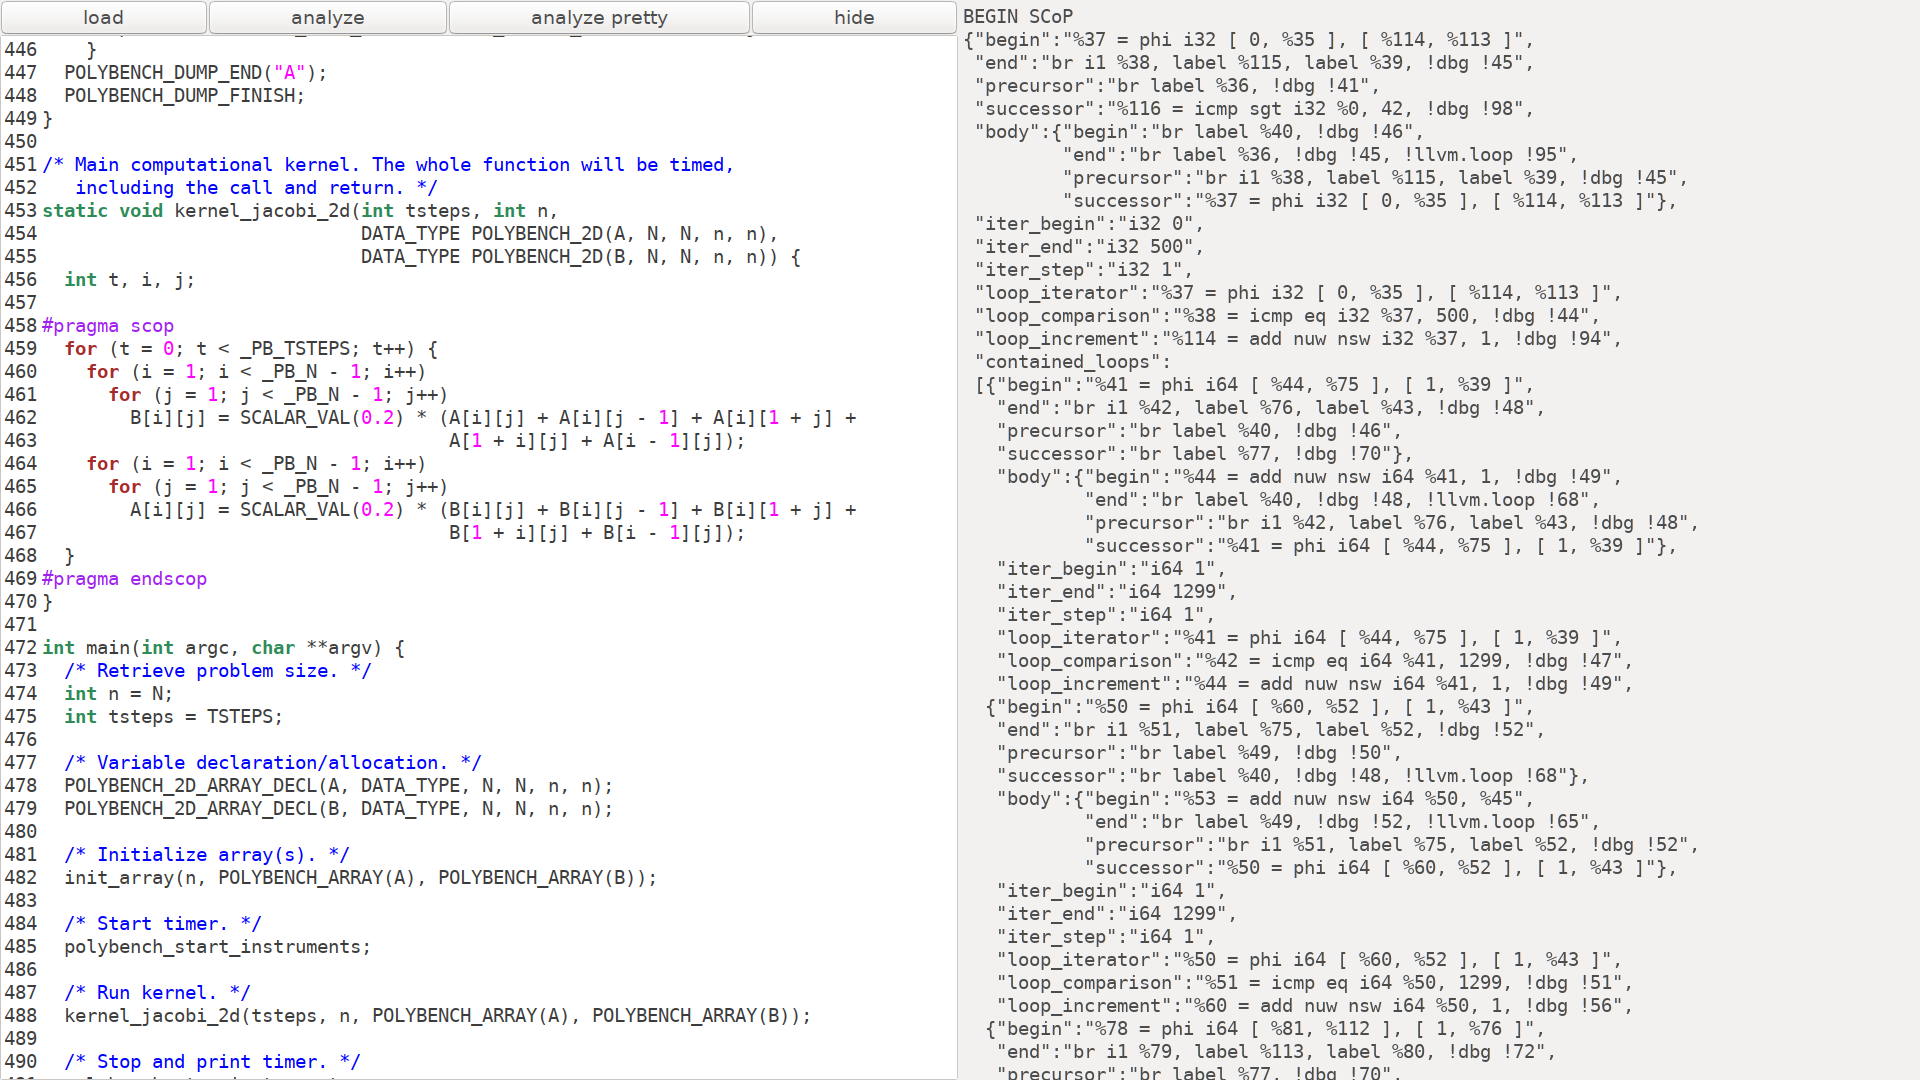
\includegraphics[width=0.9\textwidth]{figures/visual_gui2.png}
\caption{Interactive CAnDL test tool}
\medskip
\small
Left hand panel shows a SCoP in Polybench jacobi-2d, the right hand panel show the corresponding constraint solution
\label{fig:gui}
\end{figure*}

\subsection{Developer Tools}

    CAnDL makes writing compiler analysis passes easier, but reasoning about the
    semantics of compiler IR still remains difficult and the correctness of
    CAnDL programs can only be guaranteed with thorough testing.
    It is important to keep in mind that CAnDL is targeted at expert compiler
    developers.

    In order to make debugging of CAnDL programs more feasible, we developed
    supporting tools.
    Most importantly, this includes an interactive gui, where developers can
    test out corner cases of CAnDL programs to find false positives and false
    negatives.
    This gui is shown in \autoref{fig:gui}, the example is from one of the use
    cases presented in a \autoref{sec:casestudies}.

    In the left column, we can see part of a C program from the PolyBench
    benchmark suite, which implements a two-dimensional Jacobi stencil.
    The gui is configured to look for static control flow regions (SCoPs), as
    described later in one of the use cases.
    The user has clicked the ``analyze'' button, which triggered the analysis to
    run and prints the results in the right column.

    The solver found a SCoP in the IR code (corresponding to lines 459-468 of
    the C program).
    The text on the right shows the hierarchical structure of the solution, with
    IR values assigned to every variable.
    The corresponding C entities can be recovered using the debug
    information that is contained in the generated LLVM IR code.
    By modifying the C code, the developer can now test the detection and
    e.g.\ verify that no SCoP is detected if irregular control flow is
    introduced.

\section{Case Studies}
\label{sec:casestudies}

    We evaluate the usefulness of CAnDL on three real life use cases.
    We first use it  for  simple peephole optimizations.
    We then apply CAnDL to graphics shader code optimization.
    Finally, we demonstrate the detection of static control flow parts (SCoPs)
    for polyhedral code analysis.
    Where possible, we compare the number of lines of CAnDL code, the achieved
    program coverage and performance against prior approaches.

\subsection{Simple Optimizations}

    Arithmetic simplifications in LLVM are implemented in the
    \texttt{instcombine} pass.
    One example of this is the standard factorization optimization that uses the
    law of distributivity to simplify integer calculations as shown in
    \autoref{fig:factorization1}.
    It is implemented in 203 lines of code and furthermore uses supporting
    functionality provided by \texttt{instcombine}.
    \begin{align}
        a*b+a*c\rightarrow a*(b+c)
        \label{fig:factorization1}
    \end{align}

    This analysis problem can be formulated in CAnDL as shown in
    \autoref{fig:facopport}.
    The CAnDL program even captures a much larger class of opportunities for
    factorization than \texttt{instcombine}, which require to first apply
    associative and commutative laws to reorder the values.
    This is for example needed in the case of \autoref{fig:factorization2} and
    only partially supported by LLVM with the additional \texttt{reassociate}
    pass.
    \begin{align}
        a*b+c+d*a*e->a*(b+d*e)+c
        \label{fig:factorization2}
    \end{align}

\begin{figure}[t]
\begin{lstlisting}[language=CAnDL]
Constraint ComplexFactorization
( opcode{value} = add
([$\tt \land$]) {value}.args[0] = {sum1.value}
([$\tt \land$]) {value}.args[1] = {sum2.value}
([$\tt \land$]) include SumChain at {sum1}
([$\tt \land$]) {mul1.value} = {sum1.last_factor}
([$\tt \land$]) include MulChain at {mul1}
([$\tt \land$]) {mul1.last_factor} = {mul2.last_factor}
([$\tt \land$]) include SumChain at {sum2}
([$\tt \land$]) {mul2.value} = {sum2.last_factor}
([$\tt \land$]) include MulChain at {mul2})
End
\end{lstlisting}
\vspace{-0.3cm}
\caption{ComplexFactorization in CAnDL}
\label{fig:facopport}
\end{figure}

    We evaluated the program in \autoref{fig:facopport} against the default
    factorization optimization in LLVM's \texttt{instcombine} on three benchmark
    suites: the sequential C versions of NPB, the C versions of Parboil and the
    OpenMP C/C++ versions of Rodinia.
    We extended the existing LLVM \texttt{instcombine} pass such that it
    automatically reports every time that it successfully applies the
    \texttt{tryFactorization} function.  

    % NPB:     29047 loc
    % Parboil:  7358 loc
    % Rodinia: 58510 loc
    We compiled all the individual benchmark programs in the three benchmark
    suites, which consist of 94915 lines of code in total.
    For each benchmark suite, we added up all factorizations that were
    reported.
    We also measured LLVM's total compilation time.  

    We then disabled the standard LLVM optimization and instead used the CAnDL
    generated detection functionality.
    We compiled the same application programs reporting the number of
    factorizations found and again measured the total compilation time this time
    using CAnDL.
    Note that this compilation time includes all the other passes within LLVM as
    well as the CAnDL generated path.

\subsubsection{Results}
\begin{figure}[ht]
\centering
\begin{tabular}{|l||l|l|}
\hline
         & LLVM  &CAnDL \\
\hline
\hline
Lines of Code & 203 & 12 \\ \hline
Detected in NPB & 1 & 1 + 2 \\
Detected in Parboil & 0 & 0 + 1\\
Detected in  & 24 & 24 + 4\\ \hline
Total Compilation time & 152.2s & 152.2s+7.8s \\ \hline
\hline
\end{tabular}
\vspace{-0.1cm}
\caption{Factorizations LLVM vs CAnDL}
\label{fig:factorization_results}
\end{figure}

    The results are shown in \autoref{fig:factorization_results}.
    In general, the performance impact of peephole optimizations is small
    and in two of the benchmark sets we find only very small numbers.
    LLVM was unable to perform any factorization in the entire Parboil suite.
    However,  the Rodinia suite contains more opportunities, mostly in the
    Particlefilter and Mummergpu programs.

    In all three benchmarks suites, our scheme finds the same factorization
    opportunities as the \texttt{instcombine} pass plus an additional 7 cases.
    With only 12 lines of CAnDL code, we were able to capture more factorization
    opportunities than LLVM did using two hundred lines of code.

    Using CAnDL  on large complex benchmark suites only increased total
    compilation time by 5\%, demonstrating its use as a prototyping tool.

\subsection{Graphics Shader Optimizations}

    Graphics computations often involve arithmetic on vectors of single
    precision floating point values that represent either vertex positions in
    space or color values.
    Common graphics shader compilers utilize the LLVM framework using the
    LunarGLASS project.

    For real shader code, LLVM misses an opportunity for the associative
    reordering of floating point computations.
    Although such reordering is problematic in general, it is applicable in the
    domain of graphics processing.

    There are often products of multiple floating point vectors, where several
    of the factors are actually scalars that were hoisted to vectors.
    By reordering the factors and delaying the hoisting to vectors, some of the
    vector products can be simplified to scalar products, as shown in the
    following equation.
    \begin{align*}
        \vec x={}&\vec a*_v\vec b*_v\text{vec3}(c)*_v\vec d*_v\text{vec3}(e)\\
        ={}&\text{vec3}(c*e)*\vec a*_v\vec b*_v\vec d
    \end{align*}

    We implemented the required analysis functionality for this optimization
    with CAnDL, as shown in \autoref{fig:Lewis}.
    The \mbox{included} \texttt{VectorMulChain} program discovers chains of
    floating point vector multiplications in the IR code and uses the variables
    \texttt{factors} and \texttt{partials} such that
    \begin{align*}
        \text{\tt partials}[0] &= \text{\tt factors}[0]\\
        \text{\tt partials}[i+1] &= \text{\tt partials}[i]\times\text{\tt factors}[i+1].
    \end{align*}
    The \texttt{VectorMulChain} program furthermore guarantees that this is a
    chain of maximal length by checking that neither of the first two factors
    are multiplications and the last factor is not used in any multiplication.
    \texttt{ScalarHoist} detects the hoisting of scalars to vectors and this is
    used to collect all hoisted factors into the array \texttt{hoisted}.
    In a last step, all other factors are collected into the array
    \texttt{nonhoisted}.

\begin{figure}[ht]
\begin{lstlisting}[language=CAnDL]
Constraint FloatingPointAssociativeReorder
( include VectorMulChain and
([$\tt \land$]) collect j N
([$\tt \land$]) ( {hoisted[k]} = {factors[i]} forsome i=0..N
  ([$\tt \land$]) include ScalarHoist({hoisted[j]}->{out},
                       {scalar[j]}->{in})@{hoist[j]})
([$\tt \land$]) collect j N
  ( {nonhoisted[j]}  = {factors[i]} forsome i=0..N
  ([$\tt \land$]) {nonhoisted[j]} != {hoisted[i]} forall  i=0..N))
End
\end{lstlisting}
\vspace{-0.3cm}
\caption{CAnDL code for vectorized multiplication chains}
\label{fig:Lewis}
\end{figure}

    The corresponding transformation pass simply generates all the appropriate
    scalar and vector multiplications and replaces the old result with this
    newly generated one.
    We evaluated the performance impact on the CFXBench 4.0 on the  Qualcomm
    Adreno 530 GPU.

\subsubsection{Results}
    The optimization was relevant to 8 of the fragment shaders in GFXBench 4.0.
    The number of lines of code needed and the resulting performance impact are
    shown in \autoref{fig:candlshader} and \autoref{fig:qualcommspeedup}.
    A total of 19 opportunities for the optimization to be applied were
    detected.
    Although the performance impact was moderate with $1-4\%$ speedup on eight
    of the fragment shaders, it shows how new analysis can be rapidly prototyped
    and evaluated with only a few lines of code.

\begin{figure}[ht]
\centering
\begin{tabular}{|l||l|l|}
\hline
         & LLVM  &CAnDL \\
\hline
\hline
Lines of Code & Not implemented& 10 \\ \hline
Detected in GFX 4.0 & - & 19 \\ \hline
\hline
\end{tabular}
\caption{Shader optimization LLVM vs CAnDL}
\label{fig:candlshader}
\end{figure}

\begin{figure}[ht]
\centering
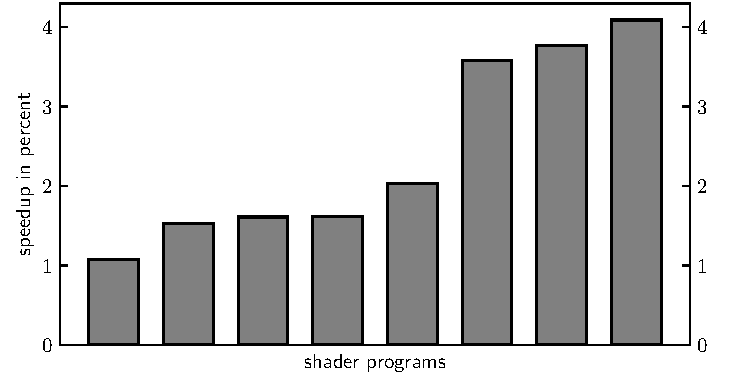
\includegraphics[width=\linewidth]{figures/qualcomm_plot.pdf}
\caption{Speedup on Qualcomm Adreno 530}
\label{fig:qualcommspeedup}
\end{figure}

\subsection{Polyhedral SCoPs}

    The polyhedral model allows compilers to utilize powerful mathematical
    reasoning to detect parallelism opportunities in sequential code and to
    implement code transformations for well structured nested
    loops.
    It is currently applicable to Static Control Flow Parts (SCoPs) with affine
    data dependencies.
    Detecting SCoPs is fundamental and a necessary first step for any later
    polyhedral optimization.

    Implementations of the polyhedral model may differ in their precise
    definition of SCoPs.
    We implemented SCoP detection functionality in CAnDL and compared against
    the Polly implementation in LLVM.
    We rely on the definition of Semantic SCoPs in \citet{Lengauer2012Polly}.
    The constraints for SCoPs can be broken into several components:

    UNDERFUL VBOX.


    \paragraph{Structured Control Flow}
    SCoPs require well structured control flow.
    Technically speaking, this means that every conditional jump within the
    corresponding piece of IR is accounted for by for loops and conditionals.
    We enforce this with the \texttt{collect} statement as demonstrated in
    \autoref{fig:collectexample}.
    We use it in CAnDL programs \texttt{ForLoop} and
    \texttt{Conditional} that describe the control flow of for loops and
    conditionals and extract the involved conditional jump instructions.
    We then use another \texttt{collect} to verify that these are indeed all
    conditional jumps within the potential SCoP.

    Once we have established the control flow, we can use the iterators that are
    involved in the loops to define affine integer computations in the loop.
    This is done in a brute force fashion with a recursive constraint program.
    Using this analysis we then check that the iteration domain of all the for
    loops is well behaved, i.e.\ the boundaries are affine in the loop
    iterators.

    \paragraph{Affine Memory Access}
    We want to make sure that all memory access in the SCoP is affine.
    For this to be true we have to verify that for each load and store
    instruction, the base pointer is loop invariant and the index is calculated
    affinely.
    The loop invariant base pointer is easily guaranteed using the
    \texttt{LocalConst} program from \autoref{fig:localconstant}.

    Checking the index calculations is more involved and is again based on the
    \texttt{collect} method that was demonstrated in
    \autoref{fig:collectexample}.
    We use the \texttt{collect} construct to find all of the affine memory
    accesses in all the loop nests.
    We then use collect all \texttt{load} and \texttt{store} instructions and
    verify that both collections are identical.

    \paragraph{}
    We evaluated our detection of SCoPs on the PolyBench suite.
    For both our method as well as for Polly, we counted how many of the
    computational kernels contained in the benchmark suite are captured by the
    analysis.

\subsubsection{Results}

    As is visible in \autoref{fig:candlvspolly}, we capture all the SCoPs that Polly
    was able to detect.
    There is some postprocessing of the generated constraint solutions required
    to achieve this.
    Firstly, our results are not in the jscop format that Polly uses but contain
    the raw constraint solution as shown on the right side of \autoref{fig:gui}.
    Also, our CAnDL implementation does not merge consecutive outer level loops
    into SCoPs of maximum size.
    To compare, we extracted the detected loops from our report
    files, manually grouped them into maximum size SCoPs and verified that they
    fully cover the SCoPs detected by Polly.

    To measure lines of code, we compared our version with the amount of code in
    Polly's \texttt{ScopDetection.cpp} pass.
    We are able to detect the same number of SCoPs with much fewer lines of
    code.
    Note that the LoC count that we give for our SCoP program does not include
    all CAnDL code involved in the detection of polyhedral regions.
    We consider the code that is not specific to this idiom (such as loop
    structures) to be part of the CAnDL standard library.
    In the same way we did not account for e.g\ the ScalarEvolution pass when
    counting the lines for Polly.

    By having a high level representation of SCoPs, we allow polyhedral compiler
    researchers to explore the impact of relaxing or tightening the exact
    definition of SCoPs in a straightforward manner, enabling rapid prototyping.


\begin{figure}[ht]
    \centering
\begin{tabular}{|l||l|l|}
\hline
         & Polly & CAnDL \\
\hline
\hline
Lines of Code & 1903 & 45 \\ \hline
Detected in datamining & 2 & 2\\
Detected in Linear-algebra & 19 & 19\\
Detected in medley & 3 & 3\\
Detected in stencils & 6 & 6\\ \hline
%Compilation time & 24.4s+37.5s & 24.4s+12.7s \\ \hline
\end{tabular}
    \label{fig:candlvspolly}
\end{figure}

\section{Related Work}

    There is a large body of work that uses constraints for program analysis.
    Constraint systems have long been used in program analysis for classical
    purposes such as dataflow analysis and type inference
    \citep{Aiken:1999:ISC:339853.339897}.
    \citet{Gulwani:2008:PAC:1375581.1375616} showed how constraints can be
    used to for some  existing analysis problems.
    It can also be used to assist generation of programs from specifications
    \citep{Srivastava:2010:PVP:1707801.1706337}.

    There is considerable work on formally verifying existing compiler
    transformations using SMT solvers and theorem provers that operate on IR
    code, among them \cite{Zhao:2012:FLI:2103656.2103709}.
    Recent domain specific language for formally verifying compiler
    optimizations, such as Alive \cite{Lopes:2015:PCP:2737924.2737965} operate
    on single static assignment compiler IR as well.
    However, it has no support for control flow and is limited to simple
    peephole optimizations.

    Further approaches to generating compiler optimizations that focus on formal
    verification instead of programmer productivity include Rhodium
    \citep{Lerner:2005:ASP:1040305.1040335}, PEC
    \citep{Kundu:2009:POC:1543135.1542513} and Gospel
    \citep{Whitfield:1997:AEC:267959.267960}.
    The CompCert tool by \citet{Mullen:2016:VPO:2908080.2908109} verifies peephole
    optimizations directly on x86 assembly code and LifeJacket
    \cite{Notzli:2016:LVP:2931021.2931024} proves the correctness of floating
    point optimizations in LLVM, as does Alive-FP \cite{Menendez2016}, which
    also generates C++ code.
    The authors of \cite{Tate:2010:GCO:1706299.1706345} investigate the
    automatic generation of optimization transformations from examples.
    None of the approaches however, tackle the issue of efficiently writing
    arbitrary compiler analysis passes.

    \citet{Martin1998} present a specification language for program analysis
    functionality called PAG that is based on abstract interpretation.
    Domain specific languages for the conception of optimization passes have
    also been studied before using tree rewrites, among them
    \citet{Olmos:2005:CSD:2136624.2136643}.
    \citet{Lipps1989} propose the domain specific language OPTRAN for matching
    patterns in attributed abstract syntax trees of Pascal programs.
    These patterns can then be automatically replaced by semantically
    equivalent, more efficient implementations. 
    Generic programming
    concepts can also be used to generate optimization passes, as
    demonstrated by \cite{Willcock:2009:RGP:1621607.1621611}.  These
    schemes however are not able to work at the IR level essential for
    compiler implementation and do not scale beyond simple functions.

    As opposed to code transformation techniques based on the LLVM ASTMatcher
    library and LibTooling \citep{be0fa11ddb194bde86a9dab8589b779c}, we work on
    compiler intermediate representation and are independent from the compiler
    frontend.
    This makes us integrate well with the existing optimization infrastructure,
    allows us to be language independent and makes our approach robust to
    shallow syntactic changes.

    Another language for implementing optimizations that emphasizes developer
    productivity is OPTIMIX \citep{Assmann1996,Assmann98optimix}, based on graph
    rewrite rules.
    OPTIMIX programs are compiled into C code that performs the specified
    transformation.
    A domain specific language for the generation of optimization
    transformations was also used in the CoSy compiler \citep{Alt1994}.
    These are simple rewrite engines and have no knowledge of global program
    constraints.

    Other work has investigated the use of constraint solvers for
    detecting structure in LLMV IR.
    \citet{ginsbach2017discovery} use a solver to detect histograms and
    scalar reductions in order to automatically parallelize code.
    A different important approach to detecting structure in intermediate
    code is the polyhedral model.
    Compilers using this model, such as
    \citet{Lengauer2012Polly}, \citet{Baskaran:2010:ACC:2175462.2175482} and
    \citet{Verdoolaege:2013:PPC:2400682.2400713}, capture well behaved
    loops with affine array accesses and are able to perform advanced loop
    optimizations.
    Recent work has investigated performant reduction computations on GPUs with
    the polyhedral model \citep{Reddy2016Reduction}.
    However this approach is not easily extensible to other program structures
    and captures only a very specific class of well behaved programs.

    In \cite{Yuan:2017:TOS:3101282.3101287}, the authors propose the use of the
    Web Ontology Language (WOL) for the description of software architectures.
    This representation enables automatic reasoning and analysis about the
    interoperability of software architectures.

\section{Conclusion}

    Optimizing compilers require sophisticated program analysis in order to
    generate performant code.
    The current way of implementing this functionality manually in programming
    languages such as C++ is not satisfactory.

    The domain specific Compiler Analysis Description Language (CAnDL) provides
    a more efficient approach.
    CAnDL programs can be used to automatically generate compiler analysis
    passes.
    They are easier to write and reduce the code size and complexity when
    comparing against manual C++ implementations.

    Although CAnDL is based on a constraint programming paradigm and uses a
    backtracking solver to analyze LLVM IR code, the use of CAnDL results in
    only moderate compile time increases.
    Many compiler analysis tasks are suitable for CAnDL, from
    peephole optimizations to sophisticated program analysis with the polyhedral
    model.

    Future work will investigate how formal verification methods can be
    applied to CAnDL in order to guarantee the correctness of compiler
    optimizations.
    Also, there is some overlap between what can be formulated in CAnDL and what
    is provided by LLVM in the form of the ScalarEvolution pass.
    We are interested as to whether we could use this existing functionality to
    speed up solving times.